\chapter{Amenity}\label{chapter-amenity}

In this chapter, we discuss how amentity might be treated in this model. 
% from Ricardo_Rent_and_Roemer_3.tex
In our base model,  an urban wage premium is the only labour attractor. Transportation costs to the urban center  determine land values. Effectively in our base model, we have set the level of amenities to zero  to focus on the productivity effects. The wage premium provides a reason to find housing in the city and to travel to the city centre to work. Housing choice, however, in reality is always the purchase of a bundle of characteristics such as location, building space, yard, local density and local \glsdisp{amenity}{amenities}. Stegman  found that ``a large majority of families who have recently moved to the suburbs are more concerned with neighborhood quality than with accessibility to other parts of the metropolitan region.'' 
``There is evidence that the amenities offered by a city enhance its growth'' \cite{clarkAmenitiesDriveUrban2002, falckPhantomOperaCultural2011a} and that amenity effects themselves scale superlinearly \cite{kraemerCulturalSustainabilityUS2022}.

Kaufmann et all \cite{kaufmannScalingUrbanAmenities2022} investigated the general statistical patterns in the quantity and spatial distribution of different urban amenities including public spaces and institutions as well as businesses, which all provide different services to urban populations, such as restaurants, parks, or universities.  They argue that amenities are in fact central for generating and supporting economic agglomeration effects, attracting investment to ``developing neighborhoods, promoting economic growth, supporting innovation clusters and facilitating businesses linkages.'' 
They show that the aggregate quantity of amenity infrastructure (not amenity supply)  in an urban area scales sub-linearly with population size across US metropolitan areas.\footnote{When they disaggregate, however, they find that for approximately 74\% of amenity types, they cannot reject linear scaling. Four percent exhibit super-linear scaling. They list take-away restaurants and travel agents in this range. Sub-linear scaling is associated with libraries, universities, and movie theatres.} This strongly suggests there are scale economies in amenity provision.\footnote{The model they use is the same as the one used to demonstrate that a scaling law holds for urban GDP. Instead of GDP, however, the dependent variable is a measure of amenity density based on data extracted from a unique new Google Places dataset, Google Places API (2012).} 


The amenities offered by a city can be seen as a form of non-market, non-monetary income \cite{kaufmannScalingUrbanAmenities2022}.  The non-market component of household incomes affects choices. Greater consumption amenities in a city will make workers willing to accept lower wages or higher rents. For firms,  lower wages mean lower costs. Thus,  higher amenity levels may lead to lower money wages as workers trade amenity for money income. With lower wages, more workers can be hired leading to higher output and a larger population \cite{pugaMagnitudeCausesAgglomeration2010}. 
When positive urban amenities prevail, rents and housing prices will be higher in larger cities, but wages may be unaffected \cite{robackWagesRentsAmenities1988, dalmazzoAmenitiesSkillbiasedAgglomeration2011}.
%localized productive advantages will make firms willing to accept higher wages and higher rents  


%It involves budget allocation. If we hold the housing budget constant and add an explicit urban amenity, other variables must adjust. 
% Higher wages make residents better off whereas higher rents make them worse off. Thus, 


%.  This helps disentangle the consumption amenities from the productive advantages of big cities.


In our base model,  To introduce amenities we can simply add an amenity value $A$ to the estimated value of any home. The value can depend on location, allowing for `better' and `worse' neighbourhoods,  and it can be made to depend on household attributes: a family with children might value a neighbourhood with a school or a park more highly. 

For some households, the amenity of an area may depend on the density of the city or of certain types in a neighbourhood. This is a social agglomeration effect that may work in addition to the agglomeration effect on production \cite{gurwitzCatastrophicAgglomeration2019} that we have already considered. There are also agglomeration effects in consumption goods. Larger consumer markets support more variety in goods and services. This variety allows a greater range of preferences to be satisfied. A larger city may have more production sectors and a larger array of consumer services, increasing the value received from a given income.  These closely related but different effects can be modeled by introducing an amenity term in various ways 

The amenity-induced rise in housing prices may absorb what would otherwise be consumption expenditure on other goods. Residents might accept smaller housing units for access to urban amenities.\footnote{Some costs may fall with agglomeration. There is evidence of a strong negative correlation between the total energy consumption of a city and its overall urban density \cite{NewmanPeterJeffrey}. Larson et al. \cite{larsonEnergyImplicationsCity2015} show that per-capita energy use is relatively invariant to city size when growth is driven by wages but falls modestly with growth induced by rising amenity.} In any case, there will be distributional effects as amenities play a larger role in urban agglomeration. Property owners will capture increased land rents. If amenities are funded out of taxes, the burden falls on all residents, since property taxes are very roughly related to housing consumption, but the land rents are captured by institutional owners as well as owner-occupiers and not by tenants.


%\glspl{amenity}, or non monetary income it another form of wealth,See Kaufmann et al. \cite{kaufmannScalingUrbanAmenities2022}.  and it is %, are however, an important feature of the urban system. 
% We have intentionally suppressed amenity but can add it it simply.
% (ownership effects, produtivity spilllovers, - table where you show them in the static and dynamci case with amentity)
% 2 classes of exploratin of the model in the past tho chaptered

 
%To understand amenity in our model, we need to understand it's relationship with growth, productivity, and agglomeration.
\subsection{Modelling amenity}

This section sketches an extension of the model to study include \gls{amenity} and suggests how it might affect results. Amenity effects can be introduced in a variety of ways. %hey might work though An economics might prefer to introduce amenity as a good in the utility function of agents.
% It might then depend on the size of the city, the size of an amenity-producing sector, the specific amenity-generating infrastructure provided by the city through taxes,  or neighbourhood effects. Each of these would take a different functional form. In our model agents are represented by their demand for housing, so the same terms would be introduced into the bid function. % In the utility framework, bids are simply derived from the utility function, so the two approaches are equivalent. %  The virtue of using the utility framework is that it begins with the question, ``What do people want?'' rather than ``What do people do?'' The first question is more productive if we want to identify different amenities that might matter.

\subsubsection{Through household utility}
The most direct way to incorporate agglomeration amenities is  to include what might be called a \gls{utility premium} for urban dwellers as non-monetary location income $\mathbb{A}(d; N), \die{\mathbb{A}}{N}> 0), \die[{\mathbb{A}}]{d}< 0)$ depending on distance, $d$ from the centre and urban population $N$. The second term can incorporate local amenities as well. A simple linear (indirect)\footnote{The indirect utility function is a function that depends on income and prices rather than goods and services.  Income does not generate utility, but it does generate utility indirectly' because it enables people to purchase goods and services.} utility function specified on broad income (net wage plus locational amenity) is convenient for illustration:

\begin{equation}VU(w,A)= \psi+ \omega-cd + \mathbb{A}(d; N) - T(d))
\label{eqn-u}
\end{equation}
where $w$  is an urban wage p, $T(d)$ is transportation cost from the centre to $d$.
\footnote{\cite{anasUrbanSpatialStructure1998} shows that a linear transportation cost will not  hold if congestion declines  with $d$.} 
 In most versions of the Alonzo model the `wage premium' is simply given in the urban wages and there is no amenity term. 


%\footnote{wage income, if all income goes to housing, or the share of wage income going to housing services.   (If we use a Cobb-Douglas utility function we would just replace $w$ with    $\alpha Y$, where $Y$ is household income and $\alpha$ is the share of total income. } Let  $T(d)=td$ be transportation cost with  $t>0$. 
 
\begin{figure}[t!b]
\begin{center}
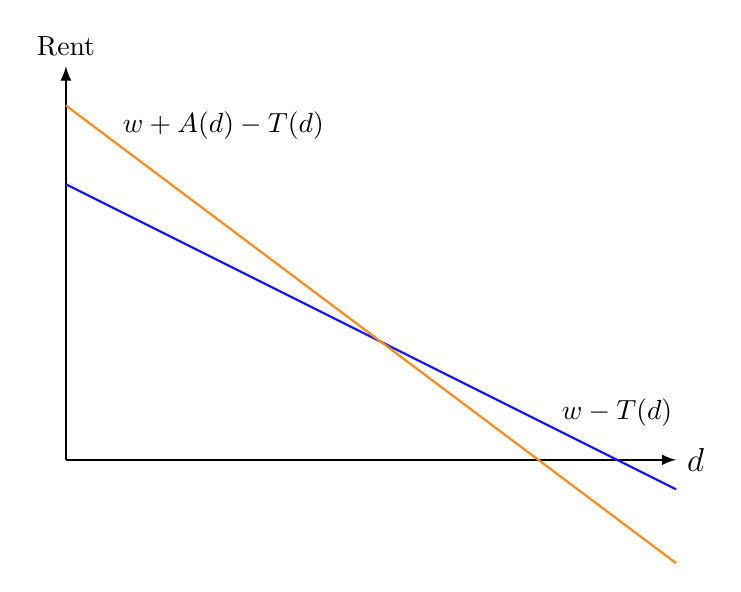
\begin{tikzpicture}[scale=.5]
\def\bndmax{5}        %https://tex.stackexchange.com/questions/68462/filling-a-complex-region-with-tikz
\def\bndmin{0.2}
\def \n {10}
\def \m {15.5}
\def \t {.5}
\def \th {1}
\def \w {7}
\tikzset{func/.style={thick,color=blue!90}}	
\draw [thick, latex-] (0,\n)node[above] {Rent}--(0,0);
\draw [thick, -latex] (0,0)--(\m,0)node[right=.25]{\large $d$};
%\foreach \xi in {0,..., \m} \draw (\xi,0)--(\xi,-.1)node[below=1]{\small$\xi$};
%\foreach \yi in {1,...,\n} \draw (0,\yi)--(-.1,\yi)node[left]{$\yi$};
%%\foreach \i in {1,4,9,16} {
	\draw[func,domain=0:\m] plot [samples=200] (\x,{\w-\t*\x});
%	\draw[func,domain=0:\m, dashed] plot [samples=200] (\x,{\w+\azero-\th*\x+\aprime*\x});

\node at (14,1.2){$w-T(d)$};
\def \azero{2}
\def \aprime {-.25}	
\tikzset{func/.style={thick,color=orange!90}}	
	\draw[func,domain=0:\m] plot [samples=200] (\x,{\w+\azero-\t*\x+\aprime*\x});
\node at (4,8.5){$w +A(d)-T(d)$};
%\node at(-.8,2) [left]{base $2^1=$};
%\node at(-.8,1) [left]{$2^0=$};
%\draw[dotted] (0,2)--(1,2)--(1,0); 
 \end{tikzpicture}
\end{center}
\caption{Rent profile with amenities}
\label{fig-amenity}
\end{figure}

 This model can produce variations on the standard result in the Alonso model. Figure~\ref{fig-amenity} illustrates a linear amenity function, $\mathbb{A}(d|N)= a-b*d$, that is convenient for illustrative purposes.  It shows how a particular amenity function might affect the rent profile, and hence city size and it allows simple experiments with the effect of increasing population on city size, wages and rents. 

In this case, amenity falls below zero in the outer regions of the city and, the geographical size of the city will be smaller. With a linear function, this happens if $\frac{a}{b} < \frac{w}{t}$. (a smaller city would have a secondary effect on wages, since with fewer workers' marginal productivity would be higher and therefore wages would rise. This would partially offset the initial decline in population.)
There would be a band of land around the city with negative amenity for commuters.\footnote{The very simple graphical result rests on several assumptions - no other housing expense, housing all the same size, wages all equal, preferences identical, transportation costs.}

The far more likely case is that $A(d) > 0$ when $w-T(d)$ falls to zero. In this case there is a band of residents around the city, outside of the population commuting to work. They do not travel to work,  do not collect a wage, but still enjoy the amenity of being close to a city. This might be a population of retired persons enjoying occasional visits and healthcare facilities.


\subsubsection{Neighbourhood amenity}
In Figure~{fig-amenity} the source of the amenity is at the centre of the city. We can easily imagine an amenity profile that is high for some neigbourhoods and lower for others, as in  In Figure~\ref{fig-amenity2}. The jagged area below the orange line is rent accruing to landowners. The variable rent comes not from a desire to be close to the source of the wage income but from household demand for local amenity.  
\begin{figure}[tb]
\begin{center}
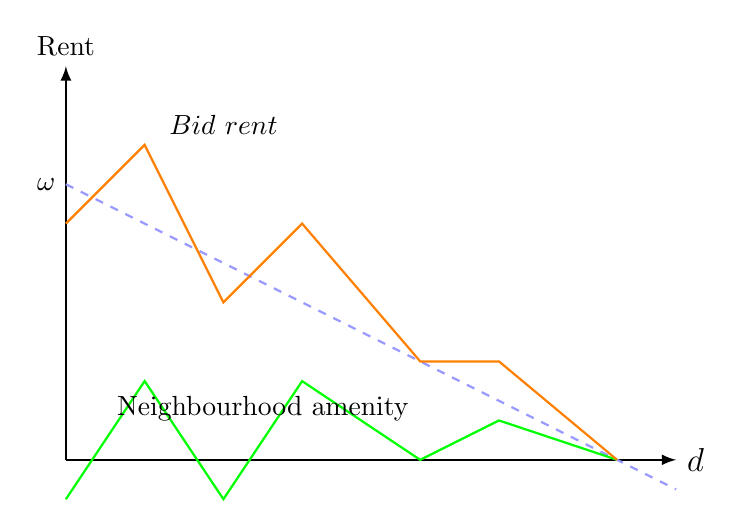
\begin{tikzpicture}[scale=.5]
\def\bndmax{5}        %https://tex.stackexchange.com/questions/68462/filling-a-complex-region-with-tikz
\def\bndmin{0.2}
\def \n {10}
\def \m {15.5}
\def \t {.5}
\def \th {1}
\def \w {7}
\tikzset{func/.style={thick,dashed, color=blue!40}}	
\draw [thick, latex-] (0,\n)node[above] {Rent}--(0,0);
\draw [thick, -latex] (0,0)--(\m,0)node[right=.25]{\large $d$};
% Basic Bid rent,
\node at(-.5,\w) {$\omega$};
\draw[func,domain=0:\m] plot [samples=200] (\x,{\w-\t*\x});
%NEIGBOURHOOD AMENITY
\draw [thick, green] (0,-1)--(2,2)--(4,-1)--(6,2)--(9,0)--(11,1)--(14,0);
\draw [thick, orange] (0,6)--(2,{7-2*.5+2})--(4,7-4*.5 -1)--(6,7-6*.5+2)--(9,7-9*.5)--(11,7-11*.5+1)--(14,7-14*.5);
\node [] at (5,1.3){Neighbourhood amenity};
\def \azero{2}
\def \aprime {-.25}	
% \tikzset{func/.style={thick,color=orange!90}}	
% 	\draw[func,domain=0:\m] plot [samples=200] (\x,{\w+\azero-\t*\x+\aprime*\x});
\node at (4,8.5){$Bid\ rent$};
%\node at(-.8,2) [left]{base $2^1=$};
%\node at(-.8,1) [left]{$2^0=$};
%\draw[dotted] (0,2)--(1,2)--(1,0); 
 \end{tikzpicture}
\end{center}
\caption{Rent profile with neighbourhood amenities}
\label{fig-amenity2}
\end{figure}
Financialization might or might not affect neighbourhood amenity. If it does it might have its effect by changing the ownership mix.

\subsubsection{Public provision of amenities}

Previous sections suggest amenities may work as a wage subsidy, potentially increasing output. Since employers will not willingly pay for urban amenities, some amenities may be financed publicly. It is common to introduce the cost of generating amenities as a tax on residents.  Since public amenities may be \glspl{public good} in the economic sense, the municipal government may be able to achieve significant wage economies with a small public expenditure.

A simple way to incorporate publicly provided amenities to make an amenity function that proportional to a fraction of public revenue, which is a fraction $\tau$ of the land value when municipalities depend on property taxes. Assuming a uniform property tax rate, total property tax revenue in a circular city are approximately $\tau(\phi+2/3 \omega)\pi \frac{\omega}{c}^2$. We can therefore include in the buyer's maximum bid function a fraction if this value. Property investors would not include this amenity component, but it would affect their decisions because amenity raises their net rent.

Notice that because amenity raises property values, in Ontario it does not raise tax revenue because the property tax rate is adjusted to balance the budget. This creates perverse incentives for municipalities \cite{blaisPerverseCitiesHidden2011}.


\subsubsection{An amenity sector}
Producing amenities takes resources. Some fraction of the workforce must be engaged in producing the amenity services. A simple approach would be to assume that the base employment that we consider demands a layer of amenities that represent the additional fraction of the population needed to provide the amenities - say 10\%  

Larger cities can support larger and more varied amenities, so that effect of amenities on property values might be larger in larger cities. At the same time, there are apparently economies of scale in the production of amenities \cite{kaufmannScalingUrbanAmenities2022}. We have no strong prior about how in amenity sector would be affected by finacialization of housing.  An effect might work through changing ownership.


\subsection{Research on amenities}
% There is a great deal of research on amenities. In this subsection mention a few that seemed noteworthy. 
Most of the literature on amenities deals with livability and the benefits for the individual. There is a strand in the literature, however, that links amenities to growth. In 1954, for example, Edward Ullman \cite{ullmanAmenitiesFactorRegional1954} published  ``Amenities as a Factor in Regional Growth,'' an article that came to be seen in the geographical literature over the following 50 years as prescient \cite{walcottCommentsEdwardUllman2010} for introducing the notion that amenities could be an important mobility magnet. 

Many have since extended this approach. Richard Florida, in a series of articles and books beginning in 2002 \cite{floridaCreativeClassEconomic2014, floridaEconomicGeographyTalent2002, floridaCompetingAgeTalent2005} examined the notion that urban growth depended on attracting the creative class and that in turn rested in part on the amenities a city offered. A 2008  Statistics Canada study, `Cities and Growth: The Left Brain of North American Cities,' Beckstead et al \ found substantial differences in average growth for cities with higher cultural employment and urban amenities.  Clark et al \cite{clarkAmenitiesDriveUrban2002} argue that much of Chicago's recent growth to 2003  should be attributed to reforms instituted by Mayor Richard M.  Daley explicitly linked to amenities and quality of life issues, including parks and schools. Abouy \cite{albouyWhatAreCities2016} finds that wage and housing cost differences across metropolitan areas are accounted for more by productivity than quality-of-life differences, however. 

Beckstead et al  \cite{becksteadCitiesGrowthLeft2008} identify amenities with the unexplained variastion in median urban house price after controlling for median household income.\footnote{  The basic premise would be that after conditioning on household income, variation in home prices across cities would be a function of the relative attractiveness of these places. The residuals yield a continuous ranking of cities based on the estimated variation in urban amenities.} Rappaport \cite{rappaportConsumptionAmenitiesCity2008} presents empirical evidence that amenities do support high-density levels, and that amenities cause approximately one-fifth of the cross-sectional variation in metro population density. 


% Molotch's (1976) metaphor suggests that the city is a machine geared to creating growth, with growth loosely defined as the intensification of land use and thus higher rent collections associated professional fees and locally based profits. Many urban economists, planners, and political scientists have made similar arguments (e.g., Bradbury, Downs, & Small, 1982; Mollenkopf, 1983; Stone, 1989). However, a quarter century later in the contemporary competition among US cities, the growth machine model has lost much of its power.
  


\newpage

